%%%%%%%%%%%%%%%%%%%%%%%%%%%%%%%%%%%%%%%%%
% Compact Academic CV
% LaTeX Template
% Version 2.0 (6/7/2019)
%
% This template originates from:
% https://www.LaTeXTemplates.com
%
% Authors:
% Dario Taraborelli (http://nitens.org/taraborelli/home)
% Vel (vel@LaTeXTemplates.com)
%
% License:
% CC BY-NC-SA 3.0 (http://creativecommons.org/licenses/by-nc-sa/3.0/)
%
%%%%%%%%%%%%%%%%%%%%%%%%%%%%%%%%%%%%%%%%%

%----------------------------------------------------------------------------------------
%	PACKAGES AND OTHER DOCUMENT CONFIGURATIONS
%----------------------------------------------------------------------------------------

\documentclass[11pt]{article} % Default document font size

%%%%%%%%%%%%%%%%%%%%%%%%%%%%%%%%%%%%%%%%%
% Compact Academic CV
% Structural Definitions
% Version 1.0 (6/7/2019)
%
% This template originates from:
% https://www.LaTeXTemplates.com
%
% Authors:
% Dario Taraborelli (http://nitens.org/taraborelli/home)
% Vel (vel@LaTeXTemplates.com)
%
% License:
% CC BY-NC-SA 3.0 (http://creativecommons.org/licenses/by-nc-sa/3.0/)
%
%%%%%%%%%%%%%%%%%%%%%%%%%%%%%%%%%%%%%%%%%

%----------------------------------------------------------------------------------------
%	REQUIRED PACKAGES AND MISC CONFIGURATIONS
%----------------------------------------------------------------------------------------

\usepackage{graphicx} % Required for including images

%\setlength{\parindent}{0pt} % Stop paragraph indentation

%----------------------------------------------------------------------------------------
%	MARGINS
%----------------------------------------------------------------------------------------

\usepackage{geometry} % Required for adjusting page dimensions and margins

\geometry{
	paper=a4paper, % Paper size, change to letterpaper for US letter size
	top=3.25cm, % Top margin
	bottom=4cm, % Bottom margin
	left=3.5cm, % Left margin
	right=3.5cm, % Right margin
	headheight=0.75cm, % Header height
	footskip=1cm, % Space from the bottom margin to the baseline of the footer
	headsep=0.75cm, % Space from the top margin to the baseline of the header
	%showframe, % Uncomment to show how the type block is set on the page
}

%----------------------------------------------------------------------------------------
%	FONTS
%----------------------------------------------------------------------------------------

\usepackage[utf8]{inputenc} % Required for inputting international characters
\usepackage[T1]{fontenc} % Output font encoding for international characters

\usepackage{ebgaramond} % Use the EB Garamond font with a reduced bold weight

%----------------------------------------------------------------------------------------
%	SECTION STYLING
%----------------------------------------------------------------------------------------

\usepackage{sectsty} % Allows changing the font options for sections in a document

\sectionfont{\fontsize{14.5pt}{18pt}\selectfont} % Set font options for sections
\subsectionfont{\bf} % Set font options for subsections
\subsubsectionfont{\mdseries\upshape\bfseries\normalsize} % Set font options for subsubsections

\newcommand{\startseclist}{\phantom{a}\vspace{-\baselineskip}}

%----------------------------------------------------------------------------------------
%	MARGIN YEARS
%----------------------------------------------------------------------------------------

\newenvironment{absolutelynopagebreak}
  {\par\nobreak\vfil\penalty0\vfilneg
   \vtop\bgroup}
  {\par\xdef\tpd{\the\prevdepth}\egroup
   \prevdepth=\tpd}

\usepackage{marginnote} % Required to output text in the margin
\newcommand{\years}[1]{\strut\marginnote{{\scriptsize #1~}$[$}}
\newcommand{\yearsplus}[1]{\strut\marginnote{{\scriptsize #1~}$\lceil$}}
\newcommand{\yearszero}{}%\strut\marginnote{$|\hspace{.1em}$}}
\newcommand{\yearsminus}{\strut\marginnote{$\lfloor$}}
\setlength{\marginparsep}{0pt} % Move the margin content closer to the text
\reversemarginpar % Margin text to be output into the left margin instead of the default right margin

%----------------------------------------------------------------------------------------
%	COLOURS
%----------------------------------------------------------------------------------------

\usepackage[usenames, dvipsnames]{xcolor} % Required for specifying colours by name

%----------------------------------------------------------------------------------------
%	LINKS
%----------------------------------------------------------------------------------------

\usepackage[bookmarks, colorlinks, breaklinks]{hyperref} % Required for links

% Set link colours
\hypersetup{
	linkcolor=blue,
	citecolor=blue,
	filecolor=black,
	urlcolor=MidnightBlue
}
 % Include the file specifying the document structure and styling
\usepackage{scrextend}

\leftskip=2em
\parindent=-1em

% Set PDF meta-information
\hypersetup{
	pdftitle={Davide Pradovera - Curriculum vit\ae},
	pdfauthor={Davide Pradovera}
}

%----------------------------------------------------------------------------------------
\pagenumbering{gobble}

\begin{document}

%----------------------------------------------------------------------------------------
%	CONTACT AND GENERAL INFORMATION
%----------------------------------------------------------------------------------------

\begin{minipage}[c]{.75\textwidth}
{\huge\bfseries Davide Pradovera} % Name
\bigskip\bigskip\medskip % Whitespace

Office 09.128, University of Vienna \\
Oskar-Morgenstern-Platz 1 \\
1090 Vienna, Austria
\medskip % Whitespace

Mobile: +41 077 95 88 993 % Mobile number
\medskip % Whitespace

Emails: \href{mailto:davide.pradovera@univie.ac.at}{davide.pradovera@univie.ac.at}\\ % Email address
\phantom{Emails: }\href{mailto:davidepradovera@gmail.com}{davidepradovera@gmail.com}\\ % Email address
\textsc{URLs}: \href{https://pradovera.github.io}{https://pradovera.github.io}\\ % Academic/personal website
\phantom{\textsc{URLs}: }\href{https://orcid.org/0000-0003-0398-1580}{https://orcid.org/0000-0003-0398-1580}\\ % Academic/personal website
\end{minipage}\hfill%
\begin{minipage}[c]{.225\textwidth}
\fbox{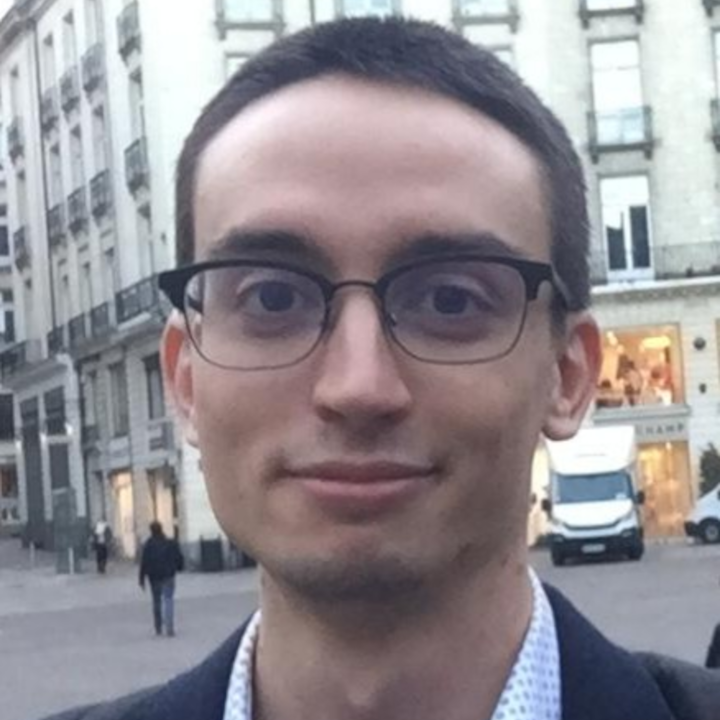
\includegraphics[width=4cm]{../images/profile}}
\end{minipage}\hfill%

\smallskip % Whitespace between contact information and specific CV information

%------------------------------------------------

Born on October 9, 1993, in Piacenza, Italy. % Date of birth

Nationality: Italian. % Nationality

%------------------------------------------------

\medskip % Whitespace between contact information and specific CV information

\section*{Current position}

\emph{University assistant and post-doctoral researcher}, Chair of Numerics of PDEs, University of Vienna. % Current or most recent employment position

%------------------------------------------------

\section*{Areas of specialization}

Numerical mathematics for partial differential equations, approximation theory, model order reduction, frequency-domain applications, scattering problems.

%----------------------------------------------------------------------------------------
%	WORK EXPERIENCE
%----------------------------------------------------------------------------------------

\section*{Appointments held}\startseclist

\years{2014--2017}{\emph{Special courses teacher}, Piacenza (I).}

\years{2016}{\emph{Developer intern}, Iren SpA, Piacenza (I).}

\years{2017--2021}{\emph{Doctoral assistant}, EPFL, Lausanne (CH).}

\years{2022}{\emph{Post-doctoral researcher}, EPFL, Lausanne (CH).}

\years{2022--now}{\emph{University assistant and post-doctoral researcher}, University of Vienna, Vienna (A).}

%----------------------------------------------------------------------------------------
%	EDUCATION
%----------------------------------------------------------------------------------------

\section*{Education}\startseclist

\years{2012--2015}{\textsc{BSc} in Applied Mathematics (\emph{cum laude}), Politecnico di Milano, Milan (I).\\
Thesis: ``A mathematical justification of the momentum operator in quantum mechanics''.\\
\phantom{m}\hfill Advisor: Prof. M. Verri.}

\years{2015--2017}{\textsc{MSc} in Computational Science and Engineering, EPFL, Lausanne (CH).\\
Project: ``Implementation of smooth contact mechanics with the mortar method''.\\
\phantom{m}\hfill Advisor: Prof. G. Anciaux.\\
Project: ``Finite elements-based Pad\'e approximants for Helmholtz frequency response problems''.\hspace{9em}\phantom{m} \hfill Advisor: Prof. F. Nobile.\\
Thesis: ``Randomized low-rank approximation of matrices and tensors''.\\
\phantom{m}\hfill Advisor: Prof. D. Kressner.}

\years{2017--2021}{\textsc{PhD} in Mathematics, EPFL, Lausanne (CH).\\
Thesis: ``Model order reduction based on functional rational approximants for parametric PDEs with meromorphic structure''.\hspace{9em}\phantom{m} \hfill Advisor: Prof. F. Nobile.}

%----------------------------------------------------------------------------------------
%	GRANTS, HONOURS AND AWARDS
%----------------------------------------------------------------------------------------

\section*{Grants, honors, and awards}\startseclist

\years{2011}{3\textsuperscript{rd} place at the ``Hong Kong International Science Fair''.}

\years{2013}{4\textsuperscript{th} place in the ``Championnat International des Jeux Math\'ematiques et Logiques''.}

\years{2014}{5\textsuperscript{th} place in the ``Championnat International des Jeux Math\'ematiques et Logiques''.}

\years{2017}{Douchet prize for best GPA, MATH-EPFL.}

\years{2020}{Prize for exceptional teaching service, Section of Mathematics, EPFL.}

\years{2021}{Junior Research Fellowship at ESI Vienna.}

%----------------------------------------------------------------------------------------
%	PUBLICATIONS AND TALKS
%----------------------------------------------------------------------------------------

\section*{Publications}

\subsection*{Journal articles}\startseclist

\years{2019}{F. Bonizzoni and DP, ``Distributed sampling for rational approximation of the acoustic scattering of an airfoil'', PAMM 19.}

\yearsplus{2020}{F. Bonizzoni, F. Nobile, I. Perugia, and DP, ``Fast Least-Squares Pad\'e approximation of problems with normal operators and meromorphic structure'', Math. Comput. 89.}

\yearszero{F. Bonizzoni, F. Nobile, I. Perugia, and DP, ``Least-Squares Pad\'e approximation of parametric and stochastic Helmholtz maps'', Adv. Comput. Math. 46.}

\yearsminus{DP, ``Interpolatory minimal rational model order reduction of parametric problems lacking uniform inf-sup stability'', SIAM J. Numer. Anal. 58.}

\yearsplus{2021}{F. Bonizzoni and DP, ``Shape optimization for a noise reduction problem by non-intrusive parametric reduced modeling'', Proc. WCCM-ECCOMAS2020.}

\yearszero{DP and F. Nobile, ``Frequency-domain non-intrusive greedy Model Order Reduction based on minimal rational approximation'', Sci. Comput. Electr. Eng. 36.}

\yearsminus{F. Nobile and DP, ``Non-intrusive double-greedy parametric model reduction by interpolation of frequency-domain rational surrogates'', ESAIM:M2AN 55.}

\years{2022}{DP and F. Nobile, ``A technique for non-intrusive greedy piecewise-rational model reduction of frequency response problems over wide frequency bands'', J. Math. Ind. 12.}

\yearsplus{2023}{F. Bonizzoni, DP, and M. Ruggeri, ``Rational-approximation-based model order reduction of Helmholtz frequency response problems with adaptive finite element snapshots'', Math. Eng. 5.}

\yearsminus{DP, ``Adaptive approximation of nonlinear eigenproblems by minimal rational interpolation'', PAMM 22 (in press).}

\subsection*{Pending articles}\startseclist

\years{2023}{DP, M. Nonino, and I. Perugia, ``Geometry-based approximation of waves in complex domains'', under review.}

\section*{Talks and attendance at events}

\subsection*{Presentations at conferences}\startseclist

\yearsplus{2019}{DP, F. Nobile, F. Bonizzoni, and I. Perugia, ``A technique for rational model order reduction of parametric problems lacking uniform inf-sup stability'', GAMM Annual Meeting 2019, Vienna (A).}

\yearszero{DP, F. Nobile, F. Bonizzoni, and I. Perugia, ``A technique for rational model order reduction of parametric problems lacking uniform inf-sup stability'', ICIAM 2019, Valencia (E).}

\yearsminus{DP and F. Nobile, ``Interpolatory rational model order reduction of parametric problems lacking uniform inf-sup stability'', \mbox{ENUMATH} 2019, Egmond aan Zee (NL).}

\yearsplus{2021}{DP, F. Nobile, and F. Bonizzoni, ``Non-intrusive model reduction of parametric frequency response problems via minimal rational interpolation'', \mbox{ICOSAHOM} 2020/2021 (virtual), Vienna (A).}

\yearsminus{DP and F. Nobile, ``Non-intrusive model reduction of parametric frequency-response problems -- with applications to UQ'', SIMAI 2020+2021, Parma (I).}

\yearsplus{2022}{DP and F. Nobile, ``Non-intrusive surrogate modeling of parametric frequency response problems -- With applications in forward UQ'', SIAM UQ22 (virtual), Atlanta (Georgia, US).}

\yearszero{DP and F. Nobile, ``Inexpensive surrogate modeling of frequency response problems by greedy minimal rational interpolation'', GAMM Annual Meeting 2022, Aachen (D).}

\yearsminus{DP and F. Nobile, ``Non-intrusive surrogate modeling of frequency response surfaces via locally adaptive sparse grids'', GIMC SIMAI Young 2022, Pavia (I).}

\subsection*{Posters}\startseclist

\yearsplus{2018}{F. Bonizzoni, I. Perugia, F. Nobile, and DP, ``An efficient algorithm for Pad\'e-type approximation of the frequency response for the Helmholtz problem'', \mbox{MoRePaS} IV, Nantes (F).}

\yearsminus{F. Bonizzoni, I. Perugia, F. Nobile, and DP, ``An efficient algorithm for Pad\'e-type approximation of the frequency response for the Helmholtz problem'', Swiss Numerics Day 2018, Zurich (CH).}

\yearsplus{2020}{DP and F. Nobile, ``Frequency-domain non-intrusive greedy Model Order Reduction based on minimal rational approximation'', SCEE 2020, Eindhoven (NL).}

\yearsminus{DP and F. Nobile, ``Frequency-domain non-intrusive greedy Model Order Reduction based on minimal rational approximation'', MORSS 2020 (virtual), Lausanne (CH).}

\years{2022}{DP and F. Nobile, ``Non-intrusive adaptive surrogate modeling of parametric frequency-response problems'', MORe 2022, Berlin (D).}

\subsection*{Other talks and seminars}\startseclist

\yearsplus{2018}{DP, F. Nobile, F. Bonizzoni, and I. Perugia, ``Fast Least-Squares Pad\'e approximation of self-adjoint problems with meromorphic structure'', seminar, \mbox{MATHICSE} retreat, Sainte-Croix (CH).}

\yearsminus{DP, F. Nobile, F. Bonizzoni, and I. Perugia, ``Fast Least-Squares Pad\'e approximation of self-adjoint problems with meromorphic structure'', workshop talk, DRWA, Alba di Canazei (I).}

\years{2019}{DP and F. Nobile, ``Polynomial approximation of resonance manifolds'', short seminar, MATHICSE retreat, Champ\'ery (CH).}

\yearsplus{2020}{DP, ``Pad\'e approximation: a quick overview'', seminar (virtual), CSQI talks, Lausanne (CH).}

\yearszero{DP, ``From Pad\'e approximation to rational interpolation'', seminar (virtual), CSQI talks, Lausanne (CH).}

\yearszero{DP, ``Minimal rational approximation'', seminar (virtual), CSQI talks, Lausanne (CH).}

\yearsminus{DP, ``Minimal rational approximation: a model reduction tool for parametrized PDEs with resonances'', seminar (virtual), PDE Afternoons, Vienna (A).}

\years{2021}{DP, ``Matching-based pMOR for dynamical systems'', seminar (virtual), CSQI talks, Lausanne (CH).}

\yearsplus{2022}{DP, ``Surrogate modeling of parametric frequency response problems via locally adaptive sparse grids'', workshop talk, ``Approximation of high-dimensional parametric PDEs in forward UQ'' ESI workshop, Vienna (A).}

\yearsminus{DP, ``Can reliable surrogate models for frequency-domain problems be both non-intrusive and cheap to build?'', workshop talk, ``UQ in kinetic and transport equations and in high-frequency wave propagation'' ESI workshop, Vienna (A).}

\subsection*{Attended events}\startseclist

\years{2018}{``Numerical Analysis of Complex PDE Models in the Sciences'' ESI workshop, Vienna (A).}

\years{2021}{Swiss Numerics Day 2021, Lausanne (CH).}

\yearsplus{2022}{``Adaptivity, High Dimensionality and Randomness'' ESI workshop, Vienna (A).}

\yearszero{Austrian Numerical Analysis Day 2022, Linz (A).}

\yearsminus{MCQMC 2022, Linz (A).}

\years{2023}{``Canonical scattering problems'' INI workshop, Cambridge (UK).}

%----------------------------------------------------------------------------------------
%	TEACHING
%----------------------------------------------------------------------------------------

\section*{Teaching experience}\startseclist

\years{2017--2021}{As teaching assistant at EPFL (preparation of course and exercise material, preparation and grading of assignments and exams):}

\bgroup
\setlength{\marginparsep}{-3mm}

\yyears{2017}{\hspace{1mm} Analyse avanc\'ee I, \textsc{BSc} in Mathematics.}

\yyears{2018}{\hspace{1mm} Analyse numerique, \textsc{BSc} in Mechanical Engineering.}

\yyears{2018}{\hspace{1mm} Analyse fonctionnelle, \textsc{BSc} in Mathematics.}

\yyears{2019}{\hspace{1mm} Introduction to partial differential equations, \textsc{BSc} in Mathematics.}

\yyears{2021}{\hspace{1mm} Numerical analysis and computational mathematics, \textsc{MSc} in Computational Sciences and Engineering.}

\yyears{2019--2021}{\hspace{1mm} Parallel and high-performance computing, \textsc{MSc} in Computational Sciences and Engineering.}
\egroup

\smallskip

\years{2022}{Invited lecturer for: Numerical methods for random PDEs and uncertainty, \textsc{PhD} course, EPFL.}

\years{2022}{As university assistant at U Vienna (charged with the organization of the whole course):}

\bgroup
\setlength{\marginparsep}{-3mm}

\yyears{2022}{\hspace{1mm} Exercises of Analysis and Linear Algebra 1, \textsc{BSc} in Mathematics.}
\egroup

\smallskip

\section*{Other service}\startseclist

\years{2019}{Supervision of \textsc{BSc} thesis: ``Approximation num\'erique du spectre des op\'erateurs elliptiques d'ordre deux'' by T. Chanay, EPFL.}

\yearsplus{2020}{Conference organizer, Model Order Reduction Summer School 2020 (virtual event).}

\yearsminus{Referee for scientific journals: Advances in Computational Mathematics.}

\yearsplus{2022}{Supervision of \textsc{MSc} project: ``Minimal rational approximation for time-harmonic Maxwell's equations'' by F. Matti, EPFL.}

\yearsminus{Referee for scientific journals: Journal of Computational Physics.}

\section*{Computer skills}\startseclist

\years{Advanced}{Matlab, C/C++, OpenMP, MPI, Python, FreeFem++, \LaTeX.}

\years{Intermediate}{CUDA, C\#, HTML.}

\years{Basic}{R, OpenFOAM, Fluent, Fortran, Java.}

%----------------------------------------------------------------------------------------
%	LANGUAGES SECTION
%----------------------------------------------------------------------------------------

\section*{Languages}\startseclist

\begin{minipage}[t]{.45\textwidth}
\begin{tabular}{rl}
Italian: & Mother tongue\\
French: & Intermediate\\
German: & Basic\\
Swedish: & Basic\\
\end{tabular}
\end{minipage}%
\begin{minipage}[t]{.45\textwidth}
\begin{tabular}{rl}
English: & Fluent\\
Japanese: & Basic\\
Spanish: & Basic\\
\\
\end{tabular}
\end{minipage}

%----------------------------------------------------------------------------------------
%	FINAL FOOTER
%----------------------------------------------------------------------------------------

% Any final footer text such as a URL to the latest version of this CV, last updated date, compiled in XeTeX, etc
\begin{center}
	\scriptsize
	\raisebox{-0.5pt}{\textbullet}~~Last updated: \today~~\raisebox{-0.5pt}{\textbullet}~~Vienna~~\raisebox{-0.5pt}{\textbullet}
\end{center}

\end{document}
